\section{Plain RNN}

As many models for text generation (and other \textit{Natural Language Processing} tasks as well) have been proposed all over the years, we decided to keep our first model as simple as possible to set a sort of lower bound that would have been useful for the successive architectures.

\begin{figure}[!htb]
    \centering
    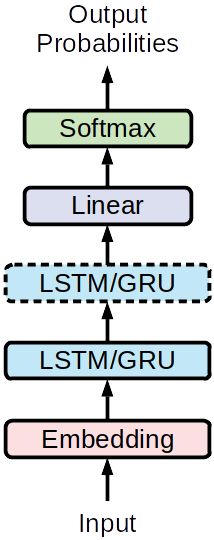
\includegraphics[scale=0.65]{images/model-1.png}%
    \caption{Plain RNN Architecture}%
    \label{plain-rnn}
\end{figure}

Therefore, inspired by Karpathy's work \parencite{karpathy2015unreasonable}, universally recognized as a milestone in the field of \textit{Natural Language Processing}, we developed the model in figure \ref{plain-rnn} consisting of an initial \textsc{Embedding} layer, mapping the tokenized input into a dense vector, which is then passed to either one or two \textsc{RNN} layer(s) and, eventually, to a final \textsc{Dense} layer, post-processed using softmax activation in order to output the probability of each token.
Given that standard \textsc{RNN} layers notoriously suffer from the so-called vanishing gradient problem, which arises in the backpropagation step, we decided to use either \textsc{LSTM} (\textsc{Long Short-Term Memory}) layers \parencite{hochreiter1997long} or \textsc{GRU} (\textsc{Gated Recurrent Units}) layers \parencite{chung2014empirical}, two special kinds of \textsc{RNN} layers developed to overcome this known problem.

Finally, as we said during the introduction of this chapter, the input and output samples we used had a fixed length, the so-called \texttt{sequence length}.
One important thing to notice is that we did not use a long sample as input and just a single token as output, but the output was instead the exact input sequence shifted by one token\footnote{
    If the input sequence is made up of the ordered set of tokens $$\{i, ..., i + sequence length - 1\}$$ taken from the \textit{Divine Comedy}, then the output is made up of the ordered set of tokens $$\{i + 1, ..., i + sequence length\}$$
}, so that the network could understand the inner patterns of the text as well.

\subsubsection{\textsc{Hyperparameters and Results}}

As we said in the introductory part of this chapter, we instantiated this architecture in three different variations, depending on the way the input text was tokenized, namely a \textit{Char-Level} model, a \textit{Word-Level} model and a \textit{Subword-Level} model.

Each of these variations had the same, independent set of hyperparameters, which we tried to tune by testing different values.
They are:
\begin{itemize}
    \item The dimension of the \textsc{Embedding} layer
    \item The kind of \textsc{RNN} (\textsc{GRU} or \textsc{LSTM})
    \item The number of \textsc{RNN} layers (either one or two), and their respective number of units
    \item The dropout rate of the \textsc{RNN} layers
\end{itemize}

After all, even though being very basic, these models were able to produce discrete results.
Taking into consideration only the configurations scoring high the \texttt{n-grams plagiarism} metric, i.e. considering only the generated samples that were not simply a copy-paste of the original \textit{Divine Comedy}, with each of the three variations we could achieve great scores (up to \textit{0.99}) in terms of \texttt{structuredness}, showing that, at least, the network had been able to understand where and how to split one tercet from the other.

As regards the structure of the verses, instead, we could achieve almost optimal results mainly with the \textit{Char-Level} and the \textit{Subword-Level} models.
In fact, while these two models were able to generate samples scoring up to \textit{0.95} in \texttt{hendecasyllabicness}\footnote{
    We remind that, using the provided code for evaluation, the first canto of the \textit{Divine Comedy} scores around \textit{0.94} in the same metric.
}, the other one could only reach a peak of \textit{0.84}, showing that it was much more difficult for it to understand the syllabication.

However, regarding the rhyming scheme, this architecture failed to get optimal results in all of its variations, reaching a maximal peak of \textit{0.38}, with an average around \textit{0.30}, similar for all of the three models.
Thus, given that, we tried to explore a more complex architecture, focusing on a way to enhance this particular aspect.